\documentclass{beamer}
\mode<presentation>
\usetheme{CambridgeUS}
\usepackage[russian]{babel}
\usepackage[utf8]{inputenc}
\usepackage[T2A]{fontenc}
\usepackage{sansmathaccent}

\usepackage{verbatim}
\usepackage{alltt}
\usepackage{minted}

\pdfmapfile{+sansmathaccent.map}
\title[Хэш-функции]{Обобщенный быстрый поиск}
\author{Наумов Д.А., доц. каф. КТ}
\date[27.04.2021] {Алгоритмы и структуры данных, 2021}

\begin{document}

%ТИТУЛЬНЫЙ СЛАЙД
\begin{frame}
  \titlepage
\end{frame}
  
%СОДЕРЖАНИЕ ЛЕКЦИИ
\begin{frame}
  \frametitle{Содержание лекции}
  \tableofcontents  
\end{frame}

\section{Обобщённый быстрый поиск}

\begin{frame}
  \frametitle{Содержание лекции}
  \tableofcontents[current]
\end{frame}
  
\begin{frame}[t]
	Двоичный поиск -- это хорошо и достаточно быстро, но можно ли искать быстрее?
	\begin{figure}[h]
		\centering
		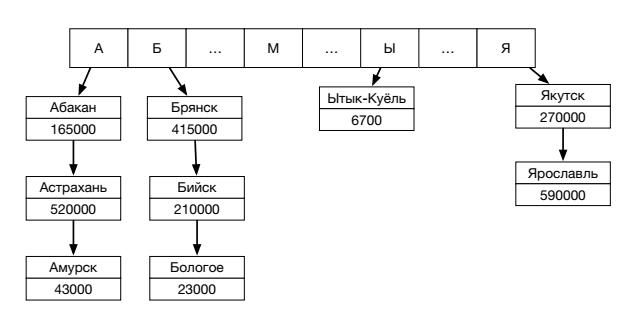
\includegraphics[scale=0.6]{images/lec08-pic01.png}
		\caption{Быстрый поиск: разбиение множества ключей на подмножества в виде связных списков}
	\end{figure}
\end{frame}

\begin{frame}[t]
	Собственно говоря, почему мы обязаны использовать именно связные списки, почему, например, не уже изученные нами деревья?
	\begin{figure}[h]
		\centering
		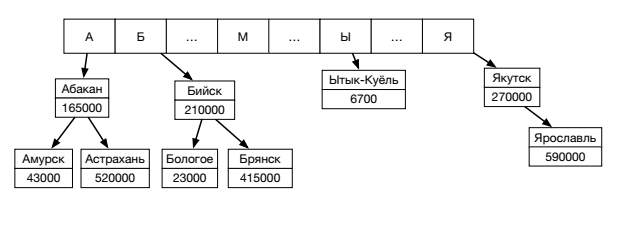
\includegraphics[scale=0.7]{images/lec08-pic02.png}
		\caption{Быстрый поиск: разбиение множества ключей на подмножества в виде деревьев поиска}
	\end{figure}
	Но такое прямолинейное разбиение не вполне хорошо -- на мягкий и твёрдый знак названий нет, для некоторых букв названий совсем мало, некоторые буквы очень популярны.
\end{frame}

\begin{frame}[t]
	\textbf{Основная идея} действительно быстрого поиска -- разбиение пространства ключей на независимые подпространства (\textit{partitioning}). При независимом разбиении на M подпространств сложность поиска уменьшается.

    \[ C \cdot O(N) \rightarrow \frac{C}{M}O(N) \]
    \[ C \cdot O(N\cdot log(N)) \rightarrow \frac{C}{M}O(N\cdot log(N)) \]
    При увеличении M время поиска уменьшается:
    \[ \lim_{K\to\infty} T(N,M) = O(1)\]
    а требуемая память увеличивается:
    \[ \lim_{K\to\infty} Mem(N,M) = \infty\]
    При $M \approx N$ имеется зона оптимальности -- поиск уже будет проводиться за $O(1)$, а вот потребная память ещё не столь велика -- $O(N)$.
\end{frame}

\begin{frame}[t]
	Примитивное разбиение пространства ключей по первым буквам -- не
очень хороший вариант. Хотелось бы иметь детерминированный способ разбиения пространства ключей на M независимых подпространств. 

    Условие разбиения -- мощность множеств ключей, принадлежащих каждому подпространству, должна быть примерно равна.

    \[ |K_1| \approx |K_2| \approx ... \approx |K_M|\]
    
    \[ \sum_{i=1}^{M} |K_i|=K\]
    
    Создаём функцию $H(K)$, удовлетворяющую некоторым условиям.
\end{frame}

\section{Хеш-функции}

\begin{frame}
  \frametitle{Содержание лекции}
  \tableofcontents[current]
\end{frame}

\begin{frame}[t]
    \begin{block}{Хеш-функция}
        есть функция преобразования множество ключей $K$ на множество $V$ мощностью $M$.
        \[H(K)\to V\]
        \[|D(V)|=M\]
        
    \end{block}
    
	Введём понятие \textbf{соперника}, того, кто предоставляет нам ключи. 
	\begin{itemize}
	    \item Цель соперника -- предоставлять ключи таким образом, чтобы значения функции оказались не равновероятными.
	    \item Соперник знает хеш-функцию и может выбирать ключи.
	\end{itemize}
\end{frame}

\begin{frame}[t]
    Чтобы быть независимыми от соперника -- и для удобства практического применения, хотелось бы для функции H(K) обеспечить следующие свойства:

	\begin{itemize}
	    \item \textbf{Эффективность} -- время вычисления хеш-функции не должно быть велико.
	    \[T(H(K)) \leq O(L(K))\]
	    где L(K) -- мера длины ключа K. 
	    \item \textbf{Равномерность} -- Каждое выходное значение равновероятно
	    \[p_{H(K_1)}=p_{H(K_2)} = \dots = p_{H(K_M)}\]
	    \item \textbf{Лавинность} -- при незначительном изменении входной последовательности выходное значение должно меняться значительно, иначе соперник может просто подобрать ключ.
	    \item Для борьбы с соперником -- \textbf{необратимость}, то есть невозможность восстановления ключа по значению его функции.
	\end{itemize}
\end{frame}

\begin{frame}[t]
    Следствия из требуемых свойств:

	\begin{itemize}
	    \item Функция не должна быть близка к непрерывной. Неплохо было бы, если бы для близких значений аргумента получались сильно различающиеся результаты.
	    \item В значениях функции не должно образовываться кластеров, множеств близко стоящих точек.
	\end{itemize}
	Примеры плохих функций:
	\begin{itemize}
	    \item $H = K2 mod 10000 для K < 100$
	    Функция монотонно возрастает. Пространство значений ключа слишком велико — и часть значений недостижима
	    \item $H =  \sum_{i=0}^{s.size-1} s[i]$ для строки s.
	    Функция даёт одинаковые значения для строк abcd и abdc и отличающиеся на единицу -- для строк abcd и abde. Сопернику легко найти
ключи, которые дают равные значения функции.
	\end{itemize}
\end{frame}

\begin{frame}[t]
    Совпадение значений функции для разных значений ключа называется \textbf{коллизией}. 

    Большое количество коллизий для данного множества ключей -- плохая хеш-функция. Конечно, без коллизий обойтись не удастся, но, если
оно больше $\frac{1}{|D(M)|}$, с хеш-функцией какие-то проблемы.

    ~
    
    Введём $H^{∗}$ -- множество хеш-функций, которые отображают пространство ключей в $m = |D(M)|$ различных значений:

    \begin{block}{Множество хеш-функций универсально}
        если для каждой пары ключей $K_i, K_j, i \noteq j$ количество хеш-функций, для которых $H^{∗}(K_i) = H^{∗}(_Kj)$ не более
        $\frac{|H^{*}|}{m}. $
    \end{block}
	При наличии такого универсального множества борьба с соперником закончится нашей победой, если мы каждый раз будем выбирать случайным образом функцию из этого множества. 
\end{frame}

\begin{frame}[t]
    Пусть множество $Z_p = \{0,1,\dots p−1\}$, множество $Z^{∗}_p = \{1,2,\dots p-1\}$, $p$ -- простое число, a $a\in Z_p^{∗}, b\in Z_p$. 
    
    ~
    
    Тогда множество $H^{∗}(p,m) = \{H(a,b,K)=((aK+b) mod p) mod m\}$ есть универсальное множество хеш-функций.

    ~ Обратим внимание на то, что для хорошей универсальной функции множество $Z_p$ есть множество неотрицательных целых чисел, что не всегда совпадает с нашими запросами
    \begin{itemize}
        \item часто требуется получить значение хешфункции (часто говорят: получить хеш) от строк, объектов и прочих сущностей. 
        \item Вполне достаточно рассматривать значение ключа как последовательность битов, только трактовать эту последовательность придётся как целое число соответствующей разрядности, то есть перейти к операциям над (N)-числами. 
        \item Для ключей с большой длиной это будет весьма неэффективно. Поэтому на практике часто применяют специальные, не универсальные хеш-функции.
    \end{itemize}
\end{frame}

\begin{frame}[t, fragile]
    Для строки можно использовать вариант полиномиальной хешфункции:

    \[h=\sum_{i=0}^{n} s_i \times q^i (mod HASHSIZE)\]
    
    \begin{minted}{c}
unsigned
hash_sum(string s, unsigned q, unsigned HASHSIZE)
{
    unsigned sum = 0;
    for (size_t i = 0; i < s.size(); i++) {
        sum = sum * q + s[i];
    }
    return sum % HASHSIZE;
}
    \end{minted}
\end{frame}

\begin{frame}[t, fragile]
    Предлагается хеш-функция, основанная на идеях из теории генерации псевдослучайных чисел:
    \begin{minted}{c}
unsigned
hash_sedgewick(string s, unsigned HASHSIZE)
{
    unsigned h, i, a = 31415, b = 27183;
    for (h = 0, i = 0; i < s.size();
        i++, a = a * b % (HASHSIZE-1)) {
        h = (a * h + s[i]) % HASHSIZE;
    }
    return h;
}
    \end{minted}
    
    Лучшие по статистическим показателям функции -- хеш-функции, применяемые в криптографии. К сожалению, у них есть и свои недостатки: у них длинный код и они достаточно медленные.
\end{frame}

\begin{frame}[t, fragile]
    Одна из хороших и быстрых функций основана на полях Галуа. Это функция CRC, очень популярная в архиваторах для контроля целостности данных (есть варианты с различным количеством бит). Она использует специальную таблицу \textt{\_table[256]} и её код очень прост:
    
    \begin{minted}{c}
uint32 
crc32(uchar *ptr, unsigned length)
{
    uint32 c = 0xFFFFFFFF;
    while (length) {
        c ^= (uint32) (ptr[0]);
        c = (c >> 8) ^ _table[c & 0xFF];
        ptr++;
        length--;
    }
    return c ^ 0xFFFFFFFF;
}
    \end{minted}
    Саму таблицу \texttt{\_table} можно создать функцией генерации таблицы -- или иметь уже готовую.
\end{frame}

\begin{frame}[t]{Исследование хэш-функций}
	Каждая из картинок даёт распределение относительной встречаемости значения хеш-функции от значения аргумента. В качестве аргументов были взяты названия идентификаторов, встречающихся в одном комплексе программ примерно в 2 миллиона строк на С++ и С#. Идеальная картинка -- закрашенный прямоугольник высотой 1.
	\begin{figure}[h]
		\centering
		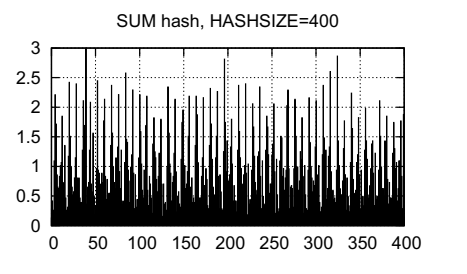
\includegraphics[scale=0.7]{images/lec08-pic03.png}
		\caption{hash\_sum для q=8, HASHSIZE принято за 400}
	\end{figure}
\end{frame}

\begin{frame}[t]
	Попробуем поменять HASHSIZE на 401.
	\begin{figure}[h]
		\centering
		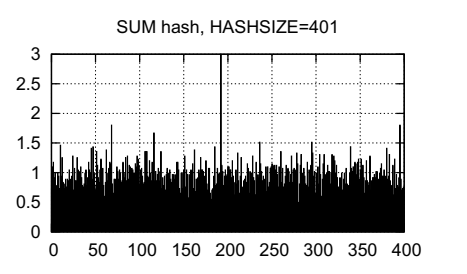
\includegraphics[scale=0.7]{images/lec08-pic04.png}
		\caption{hash\_sum для q=8, HASHSIZE принято за 401}
	\end{figure}
	А что там за пик в районе 190? Не приведёт ли он к проблемам в дельнейшем? Может и привести.
\end{frame}

\begin{frame}[t]
	Этот же набор ключей для функции hash\_sedgewick и HASHSIZE=400.
	\begin{figure}[h]
		\centering
		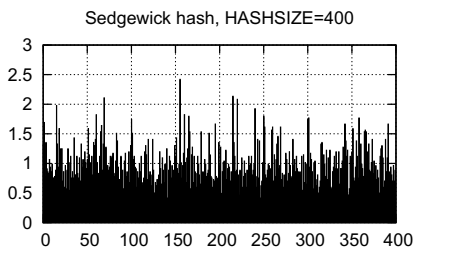
\includegraphics[scale=0.7]{images/lec08-pic05.png}
		\caption{hash\_sedgewick для q=8, HASHSIZE принято за 400}
	\end{figure}
\end{frame}

\begin{frame}[t]
	Этот же набор ключей для функции hash\_sedgewick и HASHSIZE=401.
	\begin{figure}[h]
		\centering
		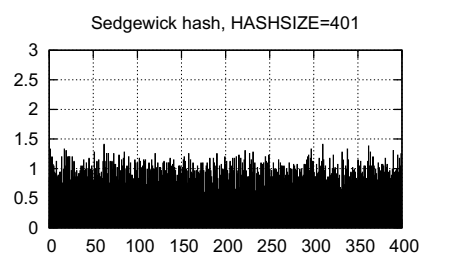
\includegraphics[scale=0.7]{images/lec08-pic06.png}
		\caption{hash\_sedgewick для q=8, HASHSIZE принято за 401}
	\end{figure}
\end{frame}

\begin{frame}[t]
	Попробуем hash\_crc для HASHSIZE, равном 400.
	\begin{figure}[h]
		\centering
		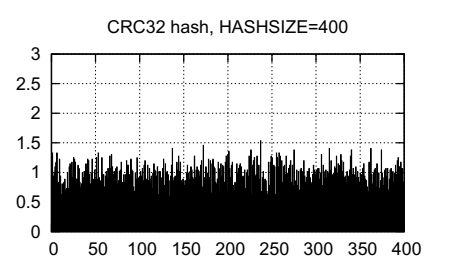
\includegraphics[scale=0.7]{images/lec08-pic07.png}
		\caption{hash\_crc для HASHSIZE=400}
	\end{figure}
\end{frame}

\begin{frame}[t]
	Попробуем hash\_crc для HASHSIZE, равном 401.
	\begin{figure}[h]
		\centering
		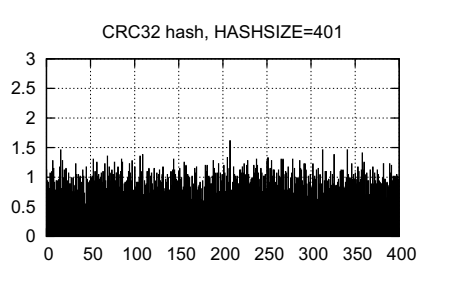
\includegraphics[scale=0.7]{images/lec08-pic08.png}
		\caption{hash\_crc для HASHSIZE=401}
	\end{figure}
\end{frame}

\begin{frame}[t]
	Мы видим, что на результат влияет размер множества значений хешфункции (HASHSIZE). Для простого числа 401 результат почти всегда лучше, чем для составного 400. Сама хеш-функция тоже очень важна.
	
	\begin{figure}[h]
		\centering
		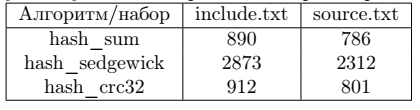
\includegraphics[scale=1]{images/lec08-pic09.png}
	\end{figure}	
	
	В таблице приведены затраты времени на исполнение программы исполнения хеш-функций для упомянутого набора идентификаторов. 
	
	Функция hash\_sedgewick оказалась самой медленной, так как для каждого символа входной строки потребовалось исполнять операцию нахождения остатка по модулю. А эта операция -- одна из самых медленных на современных компьютерах.
\end{frame}

\section{Вероятностные множества}

\begin{frame}
  \frametitle{Содержание лекции}
  \tableofcontents[current]
\end{frame}

\begin{frame}{Вероятностное множество}
    \begin{block}{Вероятностное множество}
        структура данных, реализующая функциональность абстракции <<множество>>, имеющая операции \textbf{insert} и \textbf{find} с отсутствием гарантии точности результата поиска в этом множестве. 
    \end{block}
    \begin{itemize}
        \item Результаты поиска могут быть ложноположительными, если элемент отсутствует, но операция find вернула истину. 
        \item Отсутствие элемента всегда определяется точно, то есть ложноотрицательных результатов быть не может.
    \end{itemize}
\end{frame}

\begin{frame}
    \begin{block}{Фильтр Блума}
        один из вариантов реализации вероятностных множеств. В основе его представления лежит битовый массив из $m$ бит, и для его функционирования требуется $n$ различных хеш-функций $h_1, \dots, h_n$, равномерно отображающих входные ключи на номера битов (от $0$ до $m−1$).
    \end{block}
	\begin{figure}[h]
		\centering
		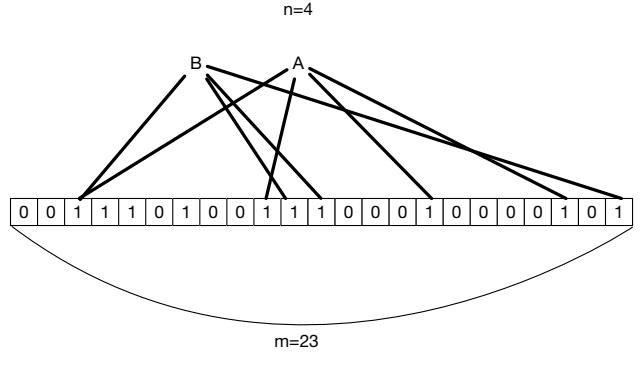
\includegraphics[scale=0.3]{images/lec08-pic10.png}
		\caption{Фильтр Блума: внесены ключи A и B}
	\end{figure}
    \begin{itemize}
        \item Операция \textbf{insert(key)}: вычисляются все n хеш-функций от key — и устанавливаются соответствующие биты в массиве.
    \end{itemize}	
\end{frame}

\begin{frame}
    \begin{itemize}
        \item При операции find вычисляются все n хеш-функций. Если хотя бы один бит в массиве не присутствует, то мы точно знаем, что такого элемента НЕТ — если бы он был, все биты, соответствующие хеш-функциям, были бы установлены. А если совпали все биты, то ответ: МОЖЕТ БЫТЬ — вполне могло оказаться, что биты установлены другими ключами.
    \end{itemize}
	\begin{figure}[h]
		\centering
		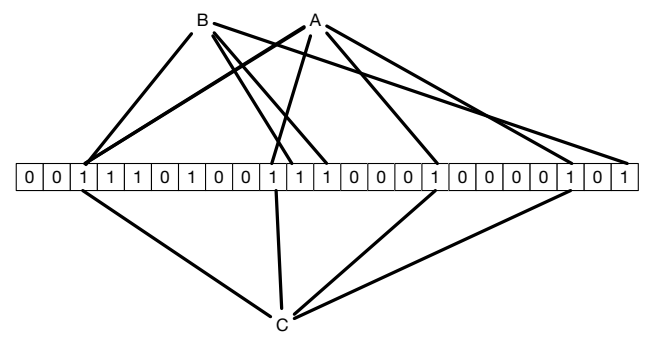
\includegraphics[scale=0.5]{images/lec08-pic11.png}
		\caption{Фильтр Блума: ключ С дает ответ МОЖЕТ БЫТЬ}
	\end{figure}
\end{frame}

\section{Хэш-таблицы}

\begin{frame}
  \frametitle{Содержание лекции}
  \tableofcontents[current]
\end{frame}

\begin{frame}{Хэш-таблицы}
    \begin{itemize}
        \item Простая хеш-таблица есть массив пар \textit{\{ключ,значение\}}.   \item Пусть размер этого массива будет HASHSIZE, и хеш-функция от ключа будет давать числа в диапазоне [0..HASHSIZE). 
        \item Тогда применение хеш-функции к ключу даст нам индекс в этом массиве, который поможет нам найти пару  \textit{\{ключ,значение\}}.
    \end{itemize}
    Каким образом мы будем искать эту пару далее, зависит от организации \textbf{хеш-таблицы}.
    
    \begin{block}{Коэффициент заполнения}
        Если известны количество элементов в контейнере $C$ и размер массива $M$, то $\alpha=\frac{C}{M}$ -- коэффициент заполнения, \textit{fill-factor} или \textit{load-factor} 
    \end{block}
    $\alpha$ -- главный показатель хеш-таблицы.
\end{frame}        

\begin{frame}
	\begin{figure}[h]
		\centering
		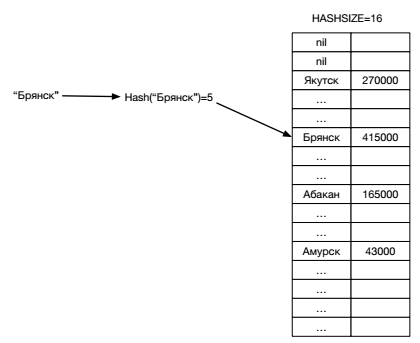
\includegraphics[scale=0.75]{images/lec08-pic12.png}
		\caption{Пример хэш-таблицы}
	\end{figure}
\end{frame}

\begin{frame}
	\begin{figure}[h]
		\centering
		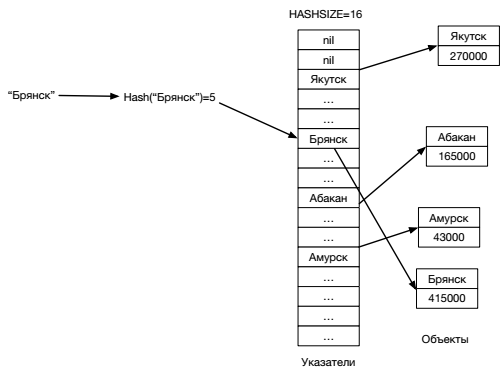
\includegraphics[scale=0.75]{images/lec08-pic13.png}
		\caption{Хеш-таблица с хранением указателей на пары ключ/значение}
	\end{figure}
\end{frame}

\begin{frame}{Хэш-таблицы}
    \begin{block}{Операция \textbf{create}}
        Операция create для хеш-таблицы часто имеет аргумент, равный начальному количеству элементов массива. 
        
        Массив заполняется либо nullptr, либо парами с невозможным значением ключей — нам всегда необходимо знать, свободен ли слот для размещения пары.
    \end{block}
    \begin{block}{Добавление элементов (операция \textbf{insert})}
        Добавление элементов (операция \textbf{insert}) требует поиска (операции \textbf{find}).        
        
        ~
        
        Если после нахождения значения хеш-функции от вновь прибывшего ключа оказывается, что запись с таким значением хеш-функции уже есть (например, Hash("Якутск") = 2 и Hash("Мышкин") = 2), то говорят, что произошла коллизия. 
    \end{block}    
    Коллизий хотелось бы избежать, так как без них операции поиска и вставки имели бы сложность O(1).
\end{frame} 

\begin{frame}{Хэш-таблицы с прямой адресацией}
    При коллизии во время создания элемента создаётся связный список
конфликтующих. 
	\begin{figure}[h]
		\centering
		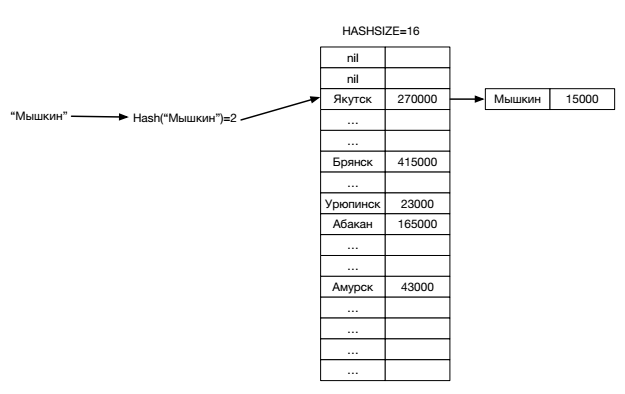
\includegraphics[scale=0.6]{images/lec08-pic14.png}
		\caption{Хеш-таблица с прямой адресацией}
	\end{figure}
\end{frame}

\begin{frame}{Хэш-таблицы с прямой адресацией}
    \begin{block}{Операция поиска и вставки}
        \begin{enumerate}
            \item При поиске вычисляется значение хеш-функции от ключа.
            \item По этому значению определяется место поиска — вторичная поисковая структура данных.
            \item Если вторичной структуры нет, то нет и элемента, который мы ищем.Теперь, если это требуется, то создаётся вторичная структура данных и элемент вставляется в неё.
            \item Иначе элемент ищется во вторичной структуре и вставляется туда при необходимости.
        \end{enumerate}
    \end{block}
\end{frame} 

\begin{frame}{Хэш-таблицы с прямой адресацией}
    \begin{block}{Операция удаления}
        \begin{enumerate}
            \item При удалении вычисляется хеш-функция от ключа.
            \item Определяется место нахождения ключа — вторичная поисковая структуре данных.
            \item Если вторичной структуры нет, то нет и элемента.
            \item Иначе элемент удаляется из вторичной структуры.
            \item Если вторичная структура пуста, удаляется сама структура и точка входа в неё.
        \end{enumerate}
    \end{block}
\end{frame} 

\begin{frame}{Хэш-таблицы с открытой адресацией}
    При другой организации хеш-таблиц вторичные структуры данных не используются — и все пары ключ/значение хранятся в самой таблице. Это означает, что требуется удобный способ разрешения коллизий. 
	\begin{figure}[h]
		\centering
		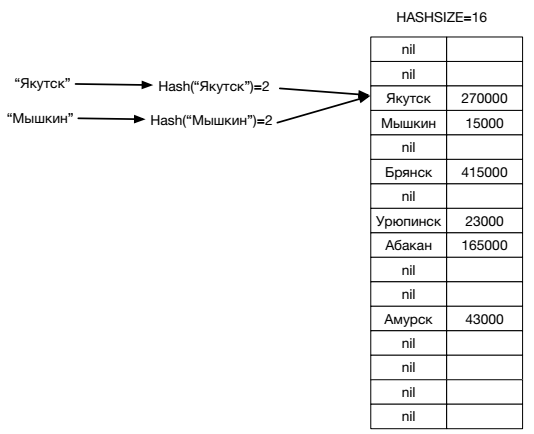
\includegraphics[scale=0.6]{images/lec08-pic15.png}
		\caption{Хеш-таблица с прямой адресацией}
	\end{figure}
\end{frame}

\begin{frame}{Хэш-таблицы с открытой адресацией}
    \begin{block}{Операция поиска по ключу}
        \begin{enumerate}
            \item При поиске существующего элемента вычисляется хеш-функция от его ключа.
            \item По значению хеш-функции определяется место поиска — индекс в хештаблице.
            \item Если по индексу ничего нет, то нет и элемента, алгоритм завершён.
            \item Иначе по индексу находится элемент с нашим ключом (требуется операция сравнения ключей)— элемент найден.
            \item Если по индексу находится элемент с другим ключом или элемент помечен удалённым, увеличиваем индекс на единицу (возвращаясь в начало таблицы при необходимости) и переходим к пункту 3.
            \item Следующий индекс вычисляется по формуле (index + 1) mod M.
        \end{enumerate}
    \end{block}
\end{frame} 

\begin{frame}{Хэш-таблицы с открытой адресацией}
    \begin{block}{Операция вставки по ключу}
        \begin{enumerate}
            \item При вставке нового элемента вычисляется хеш-функция.
            \item По значению хеш-функции определяется место поиска — индекс в хештаблице.
            \item Если по индексу находится пустой элемент или имеется элемент, помеченный как удалённый, то мы нашли подходящее место — вставляем по индексу элемент.
            \item Если по индексу уже присутствует элемент с искомым ключом — не трогая ключа, меняем данные и выходим.
            \item Если по индексу элемент с другим ключом, то индекс увеличиваем на единицу и переходим к пункту 3.
            \item Следующий индекс вычисляется по формуле (index + 1) mod M.
        \end{enumerate}
    \end{block}
\end{frame} 

\begin{frame}{Хэш-таблицы с открытой адресацией}
    \begin{figure}[h]
		\centering
		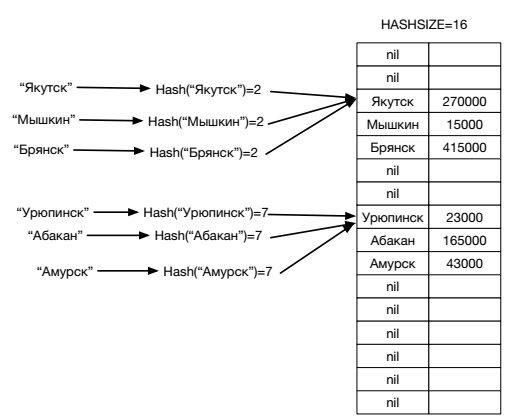
\includegraphics[scale=0.6]{images/lec08-pic16.png}
		\caption{Кластеризация коллизий}
	\end{figure}
\end{frame}

\begin{frame}{Хэш-таблицы с открытой адресацией}
    \begin{block}{Операция удаления}
        \begin{enumerate}
            \item При удалении вычисляется хеш-функция от ключа.
            \item Определяется место поиска — индекс в хеш-таблице.
            \item Если по индексу ничего нет, то нет и элемента.
            \item Иначе, если по индексу расположен элемент с требуемым ключом, то элемент найден. Помечаем его удалённым и заканчиваем алгоритм.
            \item Если по индексу расположен элемент с другим ключом, индекс увеличивается на единицу — и мы переходим к пункту 3.
            \item Следующий индекс вычисляется по формуле (index + 1) mod M.
        \end{enumerate}
    \end{block}
\end{frame} 

\begin{frame}{Хэш-таблицы с открытой адресацией}
    \begin{itemize}
        \item Мы рассмотрели простой способ нахождения пустого элемента, увеличивая номер позиции-кандидата каждый раз на единицу, K = 1 (вспомните
формулу (index+ 1) mod M). 
        \item При не очень удачной хеш-функции в таблице быстро образуются кластера из элементов, ключи которых оказались в коллизии. 
        \item Если мы обобщим эту формулу до (index+K) mod M, то, вроде бы, ничего не изменится. Но K можно сделать функцией от ключа, то есть K = H2(key). \item Оказывается, в этом случае кластеризация уменьшается, и коэффициент амортизации уменьшается вместе с ней. Это -- \textbf{рехеширование}.
    \end{itemize}
\end{frame} 

\end{document}
